% Options for packages loaded elsewhere
\PassOptionsToPackage{unicode}{hyperref}
\PassOptionsToPackage{hyphens}{url}
%
\documentclass[
]{article}
\usepackage{lmodern}
\usepackage{amssymb,amsmath}
\usepackage{ifxetex,ifluatex}
\ifnum 0\ifxetex 1\fi\ifluatex 1\fi=0 % if pdftex
  \usepackage[T1]{fontenc}
  \usepackage[utf8]{inputenc}
  \usepackage{textcomp} % provide euro and other symbols
\else % if luatex or xetex
  \usepackage{unicode-math}
  \defaultfontfeatures{Scale=MatchLowercase}
  \defaultfontfeatures[\rmfamily]{Ligatures=TeX,Scale=1}
\fi
% Use upquote if available, for straight quotes in verbatim environments
\IfFileExists{upquote.sty}{\usepackage{upquote}}{}
\IfFileExists{microtype.sty}{% use microtype if available
  \usepackage[]{microtype}
  \UseMicrotypeSet[protrusion]{basicmath} % disable protrusion for tt fonts
}{}
\makeatletter
\@ifundefined{KOMAClassName}{% if non-KOMA class
  \IfFileExists{parskip.sty}{%
    \usepackage{parskip}
  }{% else
    \setlength{\parindent}{0pt}
    \setlength{\parskip}{6pt plus 2pt minus 1pt}}
}{% if KOMA class
  \KOMAoptions{parskip=half}}
\makeatother
\usepackage{xcolor}
\IfFileExists{xurl.sty}{\usepackage{xurl}}{} % add URL line breaks if available
\IfFileExists{bookmark.sty}{\usepackage{bookmark}}{\usepackage{hyperref}}
\hypersetup{
  pdftitle={Ontario Democracy Under Pandemic: Explaining How the Ford Government Prevailed During COVID-19},
  pdfauthor={Bianca Pokhrel, Cameron Fryer, Huining Qu, Zhuoqian Li},
  hidelinks,
  pdfcreator={LaTeX via pandoc}}
\urlstyle{same} % disable monospaced font for URLs
\usepackage[margin=1in]{geometry}
\usepackage{graphicx,grffile}
\makeatletter
\def\maxwidth{\ifdim\Gin@nat@width>\linewidth\linewidth\else\Gin@nat@width\fi}
\def\maxheight{\ifdim\Gin@nat@height>\textheight\textheight\else\Gin@nat@height\fi}
\makeatother
% Scale images if necessary, so that they will not overflow the page
% margins by default, and it is still possible to overwrite the defaults
% using explicit options in \includegraphics[width, height, ...]{}
\setkeys{Gin}{width=\maxwidth,height=\maxheight,keepaspectratio}
% Set default figure placement to htbp
\makeatletter
\def\fps@figure{htbp}
\makeatother
\setlength{\emergencystretch}{3em} % prevent overfull lines
\providecommand{\tightlist}{%
  \setlength{\itemsep}{0pt}\setlength{\parskip}{0pt}}
\setcounter{secnumdepth}{-\maxdimen} % remove section numbering

\title{Ontario Democracy Under Pandemic: Explaining How the Ford Government
Prevailed During COVID-19}
\author{Bianca Pokhrel, Cameron Fryer, Huining Qu, Zhuoqian Li}
\date{2020/10/09}

\begin{document}
\maketitle

\hypertarget{excecutive-summary}{%
\section{Excecutive Summary}\label{excecutive-summary}}

With COVID-19 rampages through Ontario, the PPC (Progressive
Conservative Party) of Ontario, under the leadership of Premier Doug
Ford, achieved initial success in containing the spread of the virus,
and along with it, Ford's support rate has increased. The survey used in
the report is designed to analyze the impact of the pandemic and its
relations with the approval rate of Premier Doug Ford and his party.

Our survey, in total of 12 questions, gives us an overview of COVID-19
impact, government performance rating, and voting intentions. The survey
starts with socio-demographic questions(like gender and age) to ensure
all segments of the Ontario population are properly represented. We have
ensured to arrange the questions in a specific order so that the
previous question has minimal impact on respondents' answers. Then it is
administered using simple random sampling without replacement(SRSWOR)
through dialing random Ontario residents. The survey result was then
simulated by datasets from recently conducted polls online. The findings
have demonstrated the percentage of residents impacted by the pandemic
from each perspective. The general satisfaction with the Ford
government's response to the pandemic is around 74\%. Though the
majority of the respondents indicated that there have been no changes in
their work, financial situation, and mental health, it is extremely
concerning that about 34\% of the respondents have experienced a
negative impact on their mental health. The result above indicates that
more resources are mandatory to help Ontario residents experiencing
mental health difficulties. Several significant findings come from
respondents' voting intentions. 46.5\% of respondents would vote for the
Conservative Party if a provincial election is being held today, which
is a 7.3\% increase from the 2018 election. Moreover, 24\% of decided
voters have changed their political stands based on the government's
response to COVID. Such findings suggest that a key to gain popularity
from Ontarians is through taking proper action of the pandemic. As the
Progressive Conservative Party of Ontario passes the halfway mark of its
political term, the rising approval rate elevates the party's electoral
fortune in the 2020 election.

We have taken a quantitative approach by surveying a large sample of
randomly selected respondents. The main shortcoming of quantitative
methods is that the interpretation is not discussed thus left to the
respondent's discretion. Our survey only focuses on preconceived
issues(eg. Public health response, work, finance, mental health, vote
intentions), as a result, some other concerns may be overlooked. Our
quantitative data is simulated by the related secondary data available
online, such as Ontario census data, government statistics, and
independent research. It is confirmed that the data used is consistent,
precise, and reputable. That being said, our research is limited to the
data published, leaving our data vulnerable to slight inaccuracy without
the knowledge of the survey methodology behind the secondary data. More
specifics of the weakness will be demonstrated below. Future studies can
be conducted by distributing the survey to desired respondents with more
detailed questions aiming to help residents of Ontario improve their
situation under COVID impact.

\newpage

\hypertarget{introduction}{%
\section{Introduction}\label{introduction}}

COVID-19 pandemic has impacted Ontario in various aspects. Almost
everyone has experienced a drastic change in their way of life due to
the pandemic. Some of the changes, positive or negative, have had an
important impact on their political orientation. In this report, we
designed and analyzed the survey ``Ontario COVID-19 impact'', intending
to discover the influence of COVID-19 on Ontario resident's political
stance and voting intentions.

Upon deciding our survey methodology, we have taken cost, efficiency,
responses, and bias into consideration. More of our methodology will be
discussed below. Consequently, the survey consists of socio-demographic,
COVID impacts, political stance, and voting intentions, in which we then
distributed through phone calls by simple random sampling without
replacement (details of the survey attached to appendix). Such
probability sampling technique provides a projectible result, and it
allows us to apply statistical procedures to analyze data and calculate
errors.

The data is simulated using R (Link to code:
\url{https://github.com/1234567980/STA302-PS2}).Our findings have
revealed that only 53\% of respondents consider the public health
response ``appropriate'', whereas 29\% think it is insufficient. We have
also discovered the COVID-19 pandemic's impact on different aspects of
Ontario residents. In general, the majority of the population is not
heavily impacted. However, a significant proportion are undergoing
negative impacts from the pandemic in certain aspects such as mental
health and financial situation. Despite 77\% of the population being
satisfied with the Ontario government's response, there is still a lot
to be done in order to meet the residents' needs. It is important to
take action on such issues as we have discovered 21\% of decided voter's
voting intention is influenced by the pandemic. Thus, the electoral
fortune of the Progressive Conservative Party in 2022 is broadly
influenced by people's satisfaction with their response.

Our findings have some potential weaknesses and limitations that will
later be discussed in detail, as well as some achievable future studies.

\newpage

\hypertarget{methodologysampling-method}{%
\section{Methodology/Sampling method}\label{methodologysampling-method}}

The survey respondents were chosen using a simple random sample without
replacement method. Some statistical properties that using this method
brings is that the means obtained from our sample population can be
interpreted as unbiased estimators of the population mean. As mentioned
by Thompson and Wu in `Sampling Theory and Practice'(23. ``Wu'') the
sample mean and variance are design-unbiased estimators for the
population mean and variance. Thus by using SRSWOR we can assume in the
discussion that the analysis obtained from the survey results is
applicable for the population. Our sampling frame is Ontario residents
aged 18 years and above as our main focus is past and future voters.
Petit Poll selects a random digits sample of both land lines and phone
numbers start with Ontario area code. With around 80\% of cellphone
numbers and 20\% of land lines.The approach of using both land line and
cellphone numbers ensures we have representatives of adults who have
either access. We would randomly generate the last four digits of
numbers, ensuring that our sample covers both listed and unlisted
numbers. The sample is designed to be completely random, each with equal
probability 1/N (N = the current population of Ontario = 14,745,040)
representing all populations of Ontario. If the number is checked being
in use, we would then list it into our sample size before dialing,
ensuring that the numbers generated do not repeat. After we have
completed our desired amount of 7700 numbers, we would start the
interviewing process.

In our approach, we have referenced the interview method of land lines
from PewReseach(15. ``NW, 1615\ldots{}''). In their approach of
interviewing household through land lines, they would ``randomly ask
half the sample if they could speak with ``the youngest male, 18 years
of age or older, who is now at home'' and the other half of the sample
to speak with ``the youngest female, 18 years of age or older, who is
now at home.'' If there is no eligible person of the requested gender
currently at home, interviewers ask to speak with the youngest adult of
the opposite gender, who is now at home.''(15. ``NW, 1615\ldots{}''). We
have chosen to reference their method as it is a polished approach to
improve the proportion of young people as they are less likely to answer
and participate in surveys conducted by phone calls.

In determining our sample size, we have chosen a confidence interval of
95\%, with 5\% margin of error. Using the formula 2.7 from `Sampling
Theory and Practice'(23. ``Wu'') to calculate the desired sample size,
z-score as 1.96, standard deviation 0.5, and margin of errors 0.05, the
sample size that we hope to achieve is n = 385 with random selection of
385 people out of the total population of Ontario (N =14,745,040). As we
are only taking 0.002611\% of the population, the finite population
correction could be ignored. From the sample size above we have ensured
that we would reach the desired level of accuracy.

We have developed a few methods to manage the non-respond. It is
reported that the non-response rate of phone surveys is approximately
95\% (7. Kennedy and Hartig). To reach 385 respondents, we have aimed to
select 7700(385 x 20) Ontario residents for our survey. Secondly, at
least 3 attempts are made to complete the interview with each sampled
number on separate days. We have also planned our interview mainly in
the evening of weekdays, and daytime of weekends, to maximize the
chances of reaching potential respondents. In addition, we have
minimized the length of our survey containing only 12 most relevant
questions to our topic to further increase the completion rate, the
interview will be no longer than 3 minutes including introduction and
recording responses.

To protect respondent's privacy, the phone numbers being interviewed
will not be saved. Moreover, we avoid asking personal information such
as name or social insurance number, collecting general non-sensitive
information that will be used to weigh the sample.

In our survey, we have included socio-demographic questions including
gender and age to compensate for the bias created. We used gender and
age in our sample to compare to the population parameters from Ontario
census data from 2016(most recent census data available). Our sample is
then weighted by matching the corresponding parameters.

From the information provided above, we have estimated the cost of the
survey. Each interview takes up to three minutes, and 7700 phone calls
are made with approximately 385 respondents. Assuming each unanswered
phone call will take about one minute, and will be tried three times, it
would take roughly 387 hours to complete our interview. Thus, hiring
employees to direct the surveys at a pay rate of \$20 an hour would cost
approximately \$7,740. Assuming that \$7,740 is the monthly cost of
providing polling updates to the Progressive Conservative Party of
Ontario, the yearly cost would be \$92,880.

\hypertarget{data-preview}{%
\subsection{Data Preview}\label{data-preview}}

Below is a preview of our simulated data:

\begin{verbatim}
## # A tibble: 6 x 10
##   gender age_range who2018 q6             q7    q8    q9    q10   q11   q12  
##   <chr>  <chr>     <chr>   <chr>          <chr> <chr> <chr> <chr> <chr> <chr>
## 1 Female 55+       LIB     Just right     Okay  Good  Good  Bad   LIB   Yes  
## 2 Male   18-24     LIB     Just right     Great Good  Good  Good  PC    Yes  
## 3 Female 18-24     NDP     Too far        Okay  Good  Good  Bad   NDP   No   
## 4 Male   18-24     LIB     Not far enough Okay  Good  Bad   Good  PC    No   
## 5 Male   18-24     PC      Just right     Great Great Bad   Bad   NDP   No   
## 6 Female 55+       PC      Just right     Okay  Good  Bad   Good  PC    No
\end{verbatim}

\newpage

\hypertarget{discussion-and-results}{%
\section{Discussion and Results}\label{discussion-and-results}}

\hypertarget{public-health-response}{%
\subsection{Public Health Response}\label{public-health-response}}

Since March, confirmed cases of COVID-19 in Ontario has shown a
concerning growth. Aiming to ``flatten the curve'', the public heath
department of Ontario has responded with new policies and regulations
including physical distancing, mandatory mask or face covers, closure of
restaurants and bars, banning gatherings over 10 people. The slight
decrease on newly confirmed cases indicates that these policies are
effective. However, in our findings (Figure 1), it is shown that only
53\% of the respondents approve Public Health Ontario's approach, saying
that it is appropriate. Despite of being the majority of the population,
there are still 31\% finding the response to be inefficient, and 17\%
saying it is too extreme. Notice that public's opinion on the approach
differs for each individual, and possible bias will exist given
backgrounds of each respondent. Given two common scenarios in this case
- scenario A, a restaurant worker may think the approach to close
restaurants is too extreme, as he or she has gotten laid off. On the
contrary, one who has conceived coronavirus at his or her own workplace,
may believe the restrictions are still insufficient. Moreover, data
retrieved from ANGUSREID institute(2.``As Pandemic Endures\ldots{}'') is
from April, indicating that public opinion may vary given attributes to
the rise of COVID-19 cases recently.

\includegraphics{Pset-2-_files/figure-latex/unnamed-chunk-3-1.pdf}

Figure 1: Public opinion on health response to the current corona virus
pandemic in Ontario

\hypertarget{work-impact}{%
\subsection{Work Impact}\label{work-impact}}

From small business owners to those working in the gig economy and
artists, the government response has been lackluster as a CBC article
states that business support from the government ``is not even close to
being enough'' (13. Ore). Not only to them, but COVID-19 also has
broadly impacted almost every workers in various occupations. Some may
be temporarily discharged, others have experienced a shift from working
in the office to remotely at home. Our data from ANGUSREID Institute(19.
``So Long,\ldots) demonstrates the impact of the government's COVID-19
response on people's work.

\includegraphics{Pset-2-_files/figure-latex/unnamed-chunk-4-1.pdf}

Figure 2: COVID impact on work

In Figure 2, the findings demonstrates that 62\% of the respondents have
not seen a drastic change in their work, while 25\% of workers have
encountered positive effect by the pandemic as it has improved their
work. It is easy to over look the 13\% of respondents who has endured
negative impact on their work due to the pandemic, but the estimated
data shows 923,000 employees out of 7.1 million(8. ``Labour Market
Report\ldots{}'') has their work impaired by COVID-19. Due to the large
population size in Ontario, in spite of being only 13\%, a large amount
of Ontario residents has been experiencing difficulties in their work.

\hypertarget{financial-impact}{%
\subsection{Financial Impact}\label{financial-impact}}

Since the beginning of the pandemic, finances have been a major point of
Ontario residents' concern due to the disruption caused by the virus in
many industries. As a result, Canada's real GDP as an annualized rate
fell by 38.7\% (14. Press,\ldots) and household expenses has dropped by
13.1\%, signifying that the pandemic has had a consequential impact on
families in Canada. Both the federal and provincial governments have
offered aids to help offset the financial burden on affected families.
From emergency financial assistance to electrical bills, lots of
programs has been established as Ontario residents turn into their
leaders. We have simulated data from ANGUSREID Institute (3.
``Canadians' P\ldots{}''), hoping to determine the efficiency of
provincial government's financial support.

\includegraphics{Pset-2-_files/figure-latex/unnamed-chunk-5-1.pdf}

Figure 3: Covid19 impact on household financial needs

67.5\% of respondents have not experienced major impact on their
financial situation, as shown in Figure 3. It is pleasant to see 12.7\%
of respondents said that it has been easier to meet financial needs
since the pandemic, suggesting that the financial assistance provided by
the provincial government has been successful to some degree. However,
it is still concerning that a sizable portion of the population, 19.7\%,
has reported that their financial situations have become more difficult
as the pandemic goes on. The finding is nowhere exhaustive as the survey
question is completely self-reliant, containing no fixed standard on the
definition of ``easier'' or ``more difficult'' in terms of meeting
financial needs.

\hypertarget{mental-health-impact}{%
\subsection{Mental Health Impact}\label{mental-health-impact}}

Our findings include the impact on mental health form direct or indirect
result of this pandemic. Studies have found that financial difficulties
played a role in the increase in mental health issues as distress calls
have gone up in August due to anxieties of the termination of CERB (9.
Oct 8,..). This finding contributes to our survey results (see Figure
4), as 34\% of people reported feeling that their mental health has
gotten worse compare to prior to the pandemic. This result is confirmed
by an additional survey conducted by CTV measuring the rates of anxiety
and/or depression diagnoses during the pandemic. ``Nearly 50 percent
were considered probable candidates for anxiety disorders and more than
40 percent were likely to be clinically depressed. Almost 85 percent of
respondents reported moderate to high stress'' (20. Webber). Comparing
to the result from previous figures (see Figure 2 and Figure 3),
COVID-19 has exerted the most impact on Ontario residents' mental
health. Due to the combining issue of fear, public health regulation
(e.g.~self-isolation), impaired work, and financial difficulties, mental
health issue is to be anticipated, and should be taken in to
consideration by the provincial government. The bias of this finding
exists as there are more reasons attributed to mental health crises that
might be correlated to, but not caused by COVID-19. We are unable to
determine the percentage of such bias from the available data set.

\includegraphics{Pset-2-_files/figure-latex/unnamed-chunk-6-1.pdf}

Figure 4: Covid19 impact on mental health

\hypertarget{provincial-response}{%
\subsection{Provincial Response}\label{provincial-response}}

Findings above suggests that for the majority of Ontario residents, the
coronavirus pandemic has not impacted them in a detrimental way due to
the support from the leaders of Ontario. This is reflected by 74\% of
our respondents being satisfied with how the provincial government has
handled the pandemic, as shown in figure (5). Although the provincial
government has been successful at minimizing the negative impact of
COVID-19, there is still much room for improvement with 26\% of the
population unsatisfied. However, it is important to note that the
satisfaction rate has significantly dropped since then. A survey
conducted by ANGUSREID Institute was conducted in September and the
satisfaction rate in Ontario sank to 63\%. The decrease in satisfaction
rate in September could be attributed to the rise of COVID-19 cases that
we are currently seeing (2. ``As Pandemic Endures\ldots{}'').

\includegraphics{Pset-2-_files/figure-latex/unnamed-chunk-7-1.pdf}

Figure 5: Public satisfaction with Ontarian government's response to
COVID-19

\hypertarget{voting-intentions}{%
\subsection{Voting Intentions}\label{voting-intentions}}

From the poll conducted, we are interested to attain the voting
intentions of Ontario residents as a reflection of their satisfaction.
We have found related data from ANGUSREID institute to simulate our
sample. As a result, figure 6 demonstrates that not only has Progressive
Conservative Party under Premier Doug Ford's lead obtained a high
satisfaction rate on COVID-19 related issue - its political fortune has
also improved. 46.5\% of Ontario residents would vote for Progressive
Conservative Party if an election were held today, exceeding the second
place NDP by 18.7 points.

\includegraphics{Pset-2-_files/figure-latex/unnamed-chunk-8-1.pdf}

Figure 6: Vote intention in Ontario (Decided Voters)

Figure 7 further demonstrates the increase in popularity of the
Progressive Conservative Party through comparing the result of the 2018
provincial election. The percentage of people who would vote for
Conservatives has increased by 7.3\% from 2018, indicating not only has
the PCC maintained the majority of its supporters, it has also won
supports from voters who previously voted for other parties. Our
findings therefore enforced that the Ontario government has responded in
the right direction.

\includegraphics{Pset-2-_files/figure-latex/unnamed-chunk-9-1.pdf}

Figure 7: Percent of people who voted for PC party vs Percent of people
who would vote for PC today

We are also interested in showing the proportions of people changing
their political stance as a direct result of PPC's response of the
pandemic. Our data is simulated by finding the percentage of people has
strong opinions on the government's response and changed their vote
intentions. The approach has crucial limitations as the findings are
directly derived from the previous result. It has not taken accountable
of whether the correlation between the data sets indicates causation.
That being said, Figure 8 suggests that approximately 24\% of voters who
changed their stances are being influenced by the government's response
to the COVID-19 pandemic. Combining with the 7.3\% increase in votes,
our findings indicates that to sway the future election, PPC still has
to put effort into COVID-19 related issues such us mental health.

\includegraphics{Pset-2-_files/figure-latex/unnamed-chunk-10-1.pdf}

Figure 8: political stances and the government's response of COVID

\newpage

\hypertarget{weaknesses-and-future-studies}{%
\section{Weaknesses and Future
Studies}\label{weaknesses-and-future-studies}}

\hypertarget{limitations}{%
\subsection{Limitations}\label{limitations}}

The main topic of concern in our survey is the COVID-19 pandemic which
is currently ongoing, as a result, there were many limitations to the
data that we could find for simulating the survey responses. Due to such
issue, the choices that were available on the survey did not always
match the data that we could find. Thus, some options were grouped into
the same section during the survey design. Additionally, N/A choices
were not always included in the probabilities that could be found, as a
result some probabilities were manually scaled. Moreover, such
limitations also creates bias. We have chosen SRSWOR as our sampling
method via telephone poll, however the sources of our simulated data may
have a different survey methodology. For example, our may source of data
- Angus Reid institution conducts their survey through registered base
online survey. Furthermore, many of these sources did not disclose their
entire data set. As a result, each variable is simulated independently
based on only the reported probabilities. Thus, although we can assess
the variable independently, we are unable to determine how the variables
influence each other.

We have decided to distribute our survey using SRSWOR method. Means even
though everyone has an equal chance of being chosen, some segments of
Ontario residents might not be represented. For example, each individual
has 1/N chances of being surveyed(N being the population of Ontario).
However, Manitoulin county with a population of 13,048 will have less
chance of being represented in comparison to Toronto with the population
of 2,503,281. This shortcoming could be avoided, given enough survey
budget, by using stratified sampling method.

Our survey is aimed to obtain COVID-19 impact on Ontario residents and
their political stances. Our finding suggests that one out of five
people have changed their voting intention as a result from PPC's
response. It has proven the importance of future actions for COVID in
order to sway the upcoming election in 2022. Though we have indicated a
few area with major concerns, we cannot firmly conclude the specific
area PPC should work on to improve satisfaction rate, since it is not
the main focus of this survey. From our analysis, we have found that
22\% of people have had their financial situations negatively impacted
by the pandemic. However, it is difficult to tell whether the larger
concern is the employment rate, retirement savings, or else. It is also
laborious to determine answers to questions such as which industry is
being affected the most causing people to lose their jobs using only the
results from the survey. Furthermore, a majority of the survey answers
options rely on self-perception, which can vary by individuals. Thus the
results might be inexact.

\hypertarget{next-steps}{%
\subsection{Next Steps}\label{next-steps}}

The second wave has already caused an increase in public uncertainty and
is disrupting the approval rating of the PCC party. It is important for
Premier Doug Ford and the PPC to monitor the situation for the need to
tighten restrictions and put increased effort in improving their
approach to containing the impact of COVID-19. In future works, we will
look more in depth on the details of residents' COVID related concerns,
as an effort to help PPC identify the specific area to improve. Also we
will provide update of voting intensions and determine if it has been
impacted due to the new cases.

\newpage

\hypertarget{citations}{%
\section{Citations}\label{citations}}

\begin{enumerate}
\def\labelenumi{\arabic{enumi}.}
\item
  Allaire, JJ, et al.~Rmarkdown: Dynamic Documents for R. 2020,
  github.com/rstudio/rmarkdown. Accessed 9 Oct.~2020. R package version
  2.4.
\item
  ``As Pandemic Endures, Three-in-Ten Canadians Say Restrictions in
  Their Own Province Don't Go Far Enough.'' Angus Reid Institute, 13
  Aug.~2020, angusreid.org/covid-19-provincial-leadership/. Accessed 10
  Oct.~2020.
\item
  ``Canadians' Personal Financial Circumstances Improving, but Majority
  Will Defer Major Purchases in the next Year.'' Angus Reid Institute,
  23 July 2020, angusreid.org/covid-19-finances-spending/. Accessed 10
  Oct.~2020.
\item
  Canseco, Mario. ``Satisfaction with COVID-19 Handling Drops in Ontario
  and Quebec.'' Research Co., 19 May 2020,
  researchco.ca/2020/05/19/canada-governments-covid19/. Accessed 10
  Oct.~2020.
\item
  Government of Canada, Statistics Canada. ``2016 Census Data Tables --
  Age (in Single Years) and Average Age (127) and Sex (3) for the
  Population of Canada, Provinces and Territories, Census Divisions,
  Census Subdivisions and Dissemination Areas, 2016 Census - 100\%
  Data.'' Statcan.Gc.Ca, 2016,
  www12.statcan.gc.ca/census-recensement/2016/dp-pd/dt-td/Rp-eng.cfm?TABID=2\&LANG=E\&APATH=3\&DETAIL=0\&DIM=0\&FL=A\&FREE=0\&GC=0\&GID=0\&GK=0\&GRP=1\&PID=109525\&PRID=35\&PTYPE=109445\&S=0\&SHOWALL=0\&SUB=0\&Temporal=2016\&THEME=115\&VID=0\&VNAMEE=\&VNAMEF=\&D1=0\&D2=0\&D3=0\&D4=0\&D5=0\&D6=0.
  Accessed 10 Oct.~2020.
\item
  Hadley Wickham. Ggplot2 Elegant Graphics for Data Analysis. Cham
  Springer International Publishing, 2016. Larmarange, Joseph. Labelled:
  Manipulating Labelled Data. 2020, larmarange.github.io/labelled/.
  package version 2.7.0.
\item
  Kennedy, Courney, and Hannah Hartig. ``Response Rates in Telephone
  Surveys Have Resumed Their Decline.'' Pew Research Center, 12
  Feb.~2019,
  www.pewresearch.org/fact-tank/2019/02/27/response-rates-in-telephone-surveys-have-resumed-their-decline/.
\item
  ``Labour Market Report, August 2020.'' Ontario.Ca, Ministry of Labour,
  Training and Skills Development, 28 Sept.~2020,
  www.ontario.ca/page/labour-market-report-august-2020. Accessed 9
  Oct.~2020.
\item
  Oct 8, Janet E. Silver, and 2020 6:21pm. ``As COVID Cases Rise, so Do
  Calls for More Mental-Health Funding.'' IPolitics, 8 Oct.~2020,
  ipolitics.ca/2020/10/08/as-covid-cases-rise-so-do-calls-for-more-mental-health-funding/.
  Accessed 10 Oct.~2020.
\item
  ``Ontario Election Results From CBC News.'' CBC News,
  newsinteractives.cbc.ca/onvotes/results/.
\item
  ``Ontario Newsroom \textbar{} Salle de Presse de l'Ontario.''
  News.Ontario.Ca, 30 Sept.~2020,
  news.ontario.ca/en/release/58602/ontario-releases-updated-covid-19-modelling-for-second-wave.
  Accessed 10 Oct.~2020.
\item
  ``Ontario Spotlight: As COVID-19 Cases Climb, Can the Ford Government
  Maintain the Political Goodwill It's Earned?'' Angus Reid Institute,
  18 Sept.~2020, angusreid.org/ontario-government-august-2020/. Accessed
  10 Oct.~2020.
\item
  Ore, Jonathan. ``Mixed Reception to Feds' COVID-19 Response among
  Canadians as Pandemic Marches on \textbar{} CBC Radio.'' CBC, 12 July
  2020,
  www.cbc.ca/radio/checkup/what-grade-do-you-give-the-trudeau-government-on-covid-19-1.5643270/mixed-reception-to-feds-covid-19-response-among-canadians-as-pandemic-marches-on-1.5646508.
  Accessed 10 Oct.~2020.
\item
  Press, Jordan. ``Canadian Economy Posted Steepest Decline on Record as
  Coronavirus Struck: StatCan.'' CTVNews, 28 Aug.~2020,
  www.ctvnews.ca/business/canadian-economy-posted-steepest-decline-on-record-as-coronavirus-struck-statcan-1.5082814.
  Accessed 10 Oct.~2020.
\item
  NW, 1615 L. St, et al.~``Our Survey Methodology in Detail.'' Pew
  Research Center Methods,
  www.pewresearch.org/methods/u-s-survey-research/our-survey-methodology-in-detail/.
  Accessed 9 Oct.~2020.
\item
  R Core Team. R: A Language and Environment for Statistical Computing.
  Vienna, Austria, R Foundation for Statistical Computing, 2020,
  www.R-project.org/. Accessed 9 Oct.~2020
\item
  ``Second Wave Angst: COVID-19 Concern Levels Rebound to April Highs as
  Canadians Brace for Worse to Come.'' Angus Reid Institute, 30
  Sept.~2020, angusreid.org/covid-second-wave-september/. Accessed 10
  Oct.~2020.
\item
  Szperling, Peter. ``Anxiety Levels Increasing during COVID-19
  Pandemic: Study.'' CityTV Ottawa, 24 Sept.~2020,
  ottawa.ctvnews.ca/anxiety-levels-increasing-during-covid-19-pandemic-study-1.5119162.
  Accessed 8 Oct.~2020.
\item
  ``So Long, Office Space? Two-Thirds of Canadians Who Work from Home
  Expect It to Continue after Pandemic.'' Angus Reid Institute, 11 June
  2020, angusreid.org/coronavirus-work-from-home/. Accessed 10
  Oct.~2020.
\item
  Weber, Bob. ``COVID-19 Causing Stress, Depression and Obsessive
  Behaviour: Survey.'' CTV News, 26 Sept.~2020. Accessed 8 Oct.~2020.
\item
  Wickham, Hadley, et al.~Dplyr: A Grammar of Data Manipulation. 2020,
  dplyr.tidyverse.org, github.com/tidyverse/dplyr. Accessed 9 Oct.~2020.
\item
  Wickham, Hadley, and Jennifer Bryan. Readxl: Read Excel Files. 2019,
  readxl.tidyverse.org, github.com/tidyverse/readxl.
\item
  Wu, Changbao, and Mary E. Thompson. Sampling Theory and Practice.
  Springer.
\item
  Yihui Xie, et al.~R Markdown Cookbook.. Chapman and Hall/CRC, 2020.
\item
  Yihui Xie, et al.~R Markdown: The Definitive Guide.. Chapman and
  Hall/CRC, 2018.
\item
  Canada, Elections. ``Description of the National Register of
  Electors.'' Www.Elections.Ca, 7 July 2020,
  www.elections.ca/content.aspx?section=vot\&dir=reg/des\&document=index\&lang=e.
  Accessed 9 Oct.~2020.
\end{enumerate}

\newpage

\hypertarget{appendix}{%
\section{Appendix}\label{appendix}}

Link to code: \url{https://github.com/1234567980/STA302-PS2}

Link to
survey:\url{https://www.surveymonkey.com/r/Preview/?sm=yjJjeiM3KvfrNAOGiO2B2A4A0UKGkHgR82Qt83bwpG1fDl1g_2Fr2TY8dawJ2IdzlF}

Survey:


\includegraphics{./survey image/1.1.png}

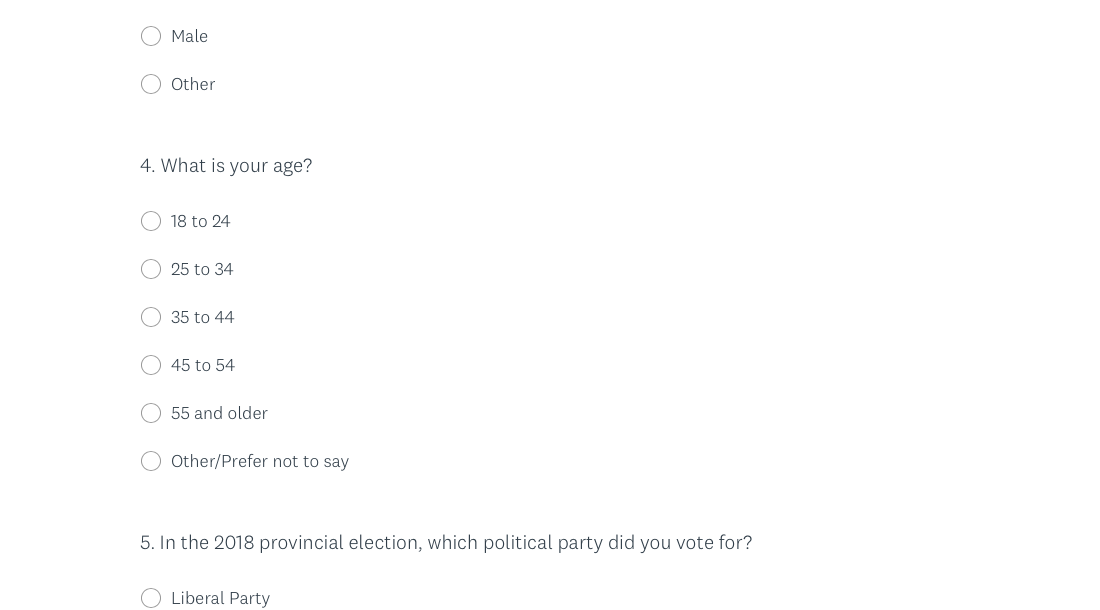
\includegraphics{./survey image/1.2.png}

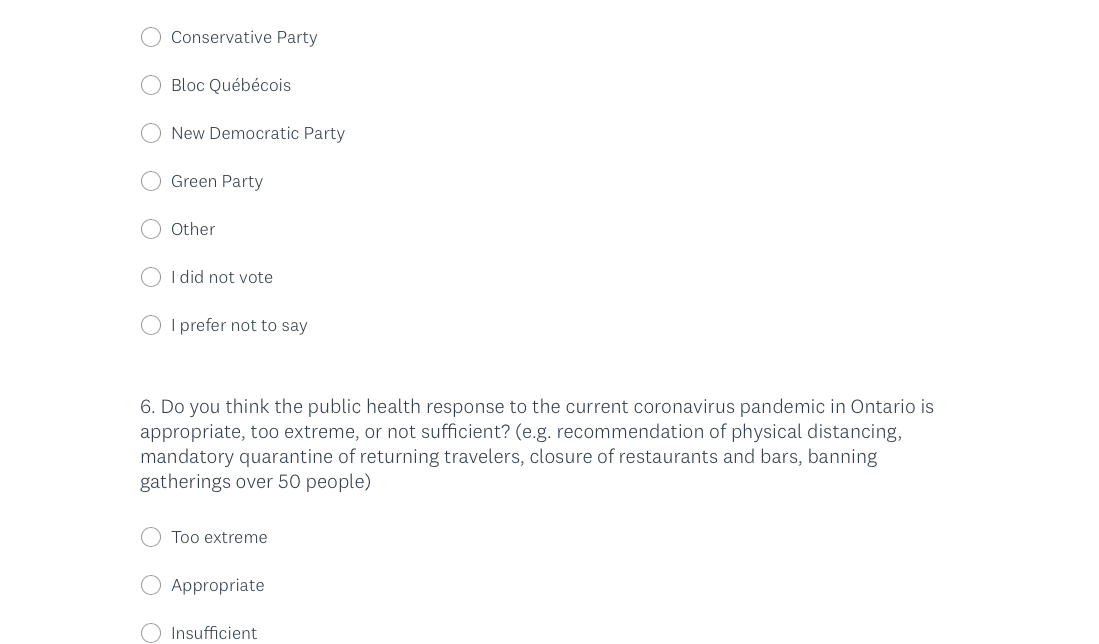
\includegraphics{./survey image/1.3.png}

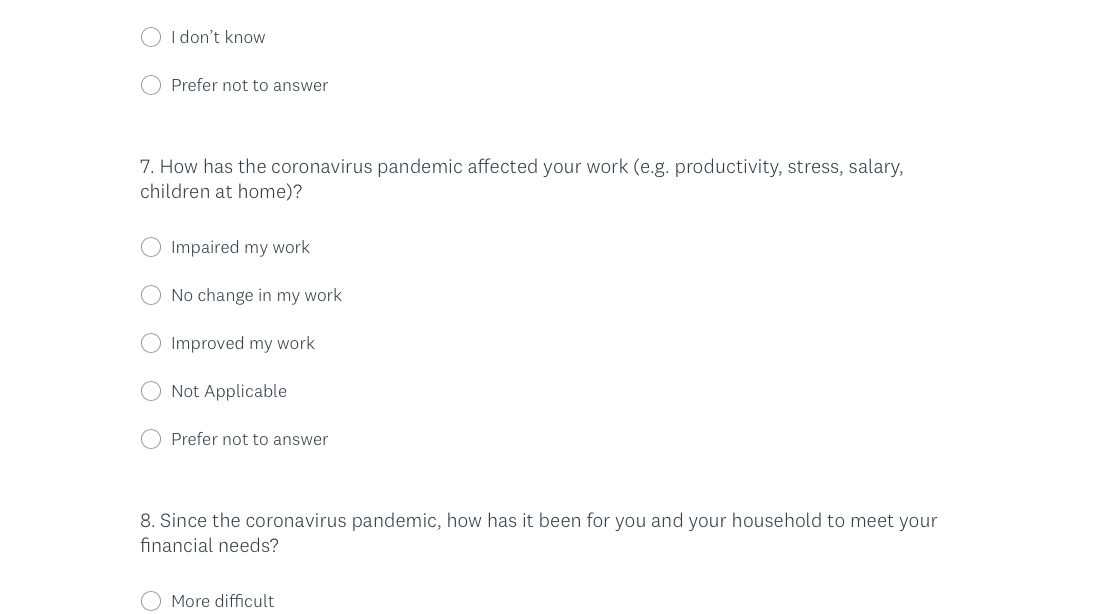
\includegraphics{./survey image/1.4.png}

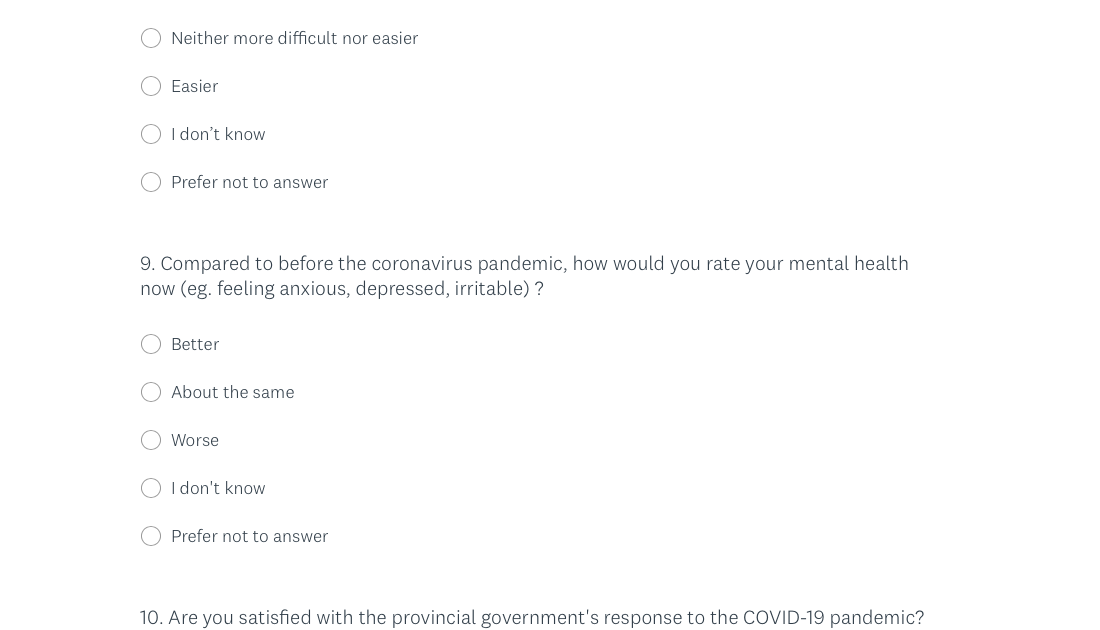
\includegraphics{./survey image/1.5.png}

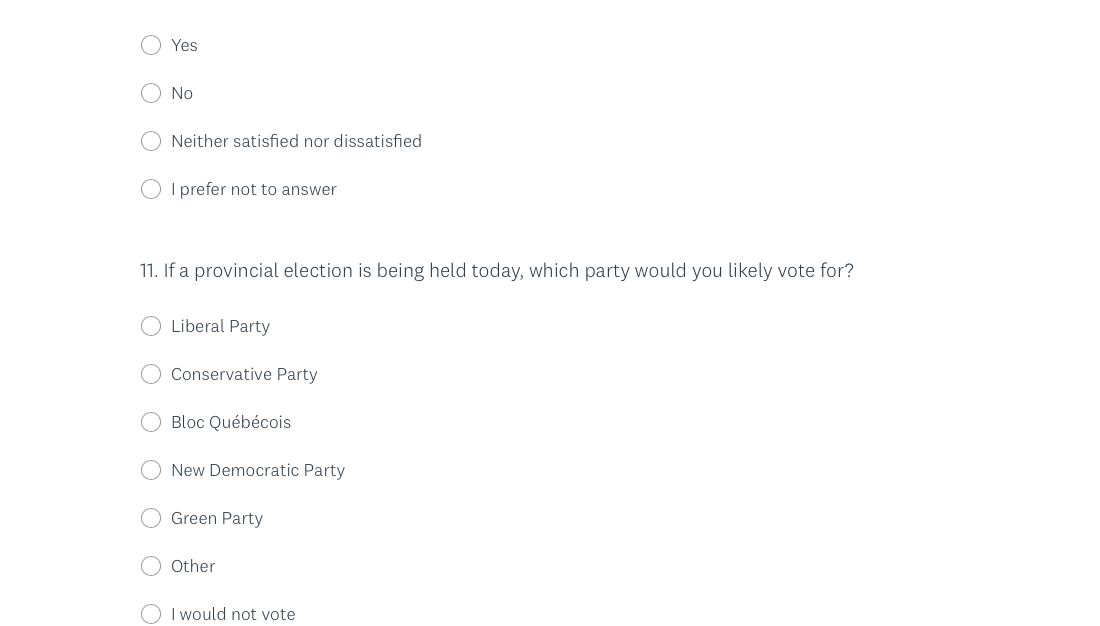
\includegraphics{./survey image/1.6.png}


\includegraphics{./survey image/1.7.png}

\end{document}
